% !TeX spellcheck = en_US
% !TeX root = ./0_article.tex

\section{Validating and completing the models}
\subsection{Validation the models}
	With the aim of verifying the soundness of the previous conclusions, we set up experiments using an actual IC composed of both triple-well and dual-well substrate on a monolithic die.
	These experiments consist in verifying if the difference in injected energy depending on the substrate type is actually significant or not.
	
	The target used is a STM32F439 microcontroller, alongside the platform presented in the first chapter.
	The IC die measures approximately 5.5 mm \texttimes\ 4.5 mm.
	We call these experiments "IC ground current mapping", and quite naturally, they consist in measuring in specific conditions the current at the target circuit external ground connection.
	The entirety of the IC is mapped, and a voltage pulse is injected at each location.
	Then, we measure the current at the circuit ground and calculate its RMS value to represent it into a two-dimensional cartography.
	% !TeX spellcheck = en_US
% !TeX root = ./0_article.tex

\begin{figure}[h]
	\centering
	\includegraphics[width=0.83\columnwidth]{./figures/stmPhotoImshow.pdf}
	\caption{Caption}
	\label{stm_ir_photo}
\end{figure}

	Knowing the coarse structure of the considered IC, in addition to having insights on the substrate type, we could draw the coarse structure picture shown in Fig. \ref{stm_ir_photo}.
	The "glue logic" regions are known to be made with triple-well substrates, while the "flash control" and "analog" regions are made with dual-well substrates.
	\textcolor{orange}{The memories, however, are made of a mix of both.}
	% !TeX spellcheck = en_US
% !TeX root = ./0_article.tex

\begin{figure}[h]
	\centering
	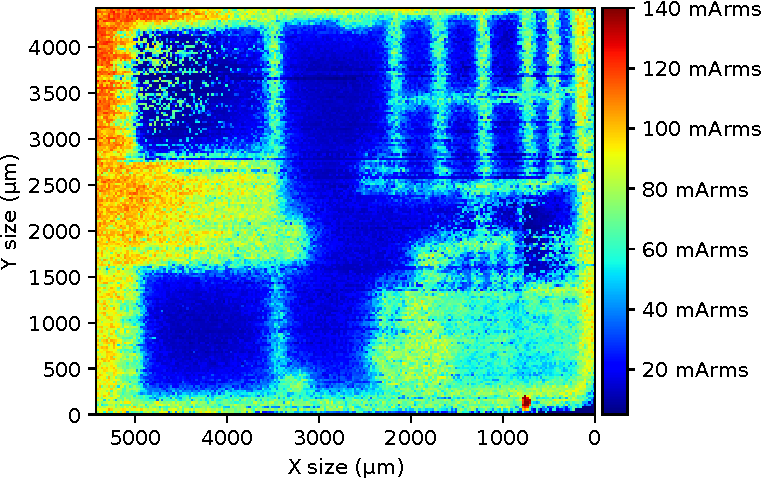
\includegraphics[width=\columnwidth]{./figures/pos_neg_IGND.pdf}
	\caption{Ground current mapping of our target IC}
	\label{stm_ignd}
\end{figure}

	The experimental results are shown in Fig. \ref{stm_ignd}, and the experimental parameters are the following:
	\begin{itemize}
		\item Negative voltage pulse of 70 V amplitude;
		\item Pulse width of 20 ns;
		\item IC substrate thickness of 50 \textmu m.
	\end{itemize}
	The voltage pulse used is of negative polarity as we have observed a very fast degradation of IC subjected to positive voltage pulses, therefore we decided to avoid them at all cost.
	When analyzing the results, we can notice significant differences in the measured current depending on various regions, and the IC floorplan seems to draw itself on the current map.
	The measured RMS current ranges from 10 mArms to 140 mArms, and as predicted by the simulation results, in the regions where the substrate is of dual-well type, the current is higher than on regions where the substrate is of triple-well type, such as the analog block or the flash control region.
	
	These observations confirm the soundness of the proposed models.
	However, as we have seen previously, these models do not consider the functional nature of the considered ICs: their logic behavior.
	To circumvent this limitation, we decided to develop an addition to the initial simulation flow, thus the name "hybrid simulation flow".

\subsection{Completing the models}
	To complete the models as they are, it is required to properly consider the logical behavior of the considered circuits, which allows for a better appreciation of BBI induced effects.
	These additional steps consist in modeling actual logic and sequential elements  in the same technology as the considered IC, and extracting the significant disturbed signals from the SCS simulation and injecting them into these devices.
	% !TeX spellcheck = en_US
% !TeX root = ./0_article.tex

\begin{figure}[h]
	\label{ivxbufmos}
	\centering
	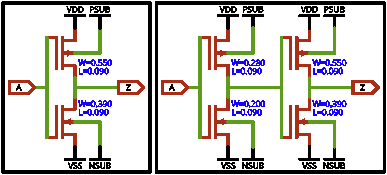
\includegraphics[width=0.5\textwidth]{./figures/IVX_BUFF_X4_3.pdf}
	\caption{IVX MOS SCH \textcolor{red}{A-T-ON LE DROIT DE METTRE CE SCHÉMA ?}}
\end{figure}

	For this purpose, we modeled an inverter, a buffer and a DFF.
	The inverter and buffer schematics, alongside the transistors sizes, are shown in Fig. \ref{ivxbufmos}.
	% !TeX spellcheck = en_US
% !TeX root = ./0_article.tex

\begin{figure}[h]
	\label{dffmos}
	\center
	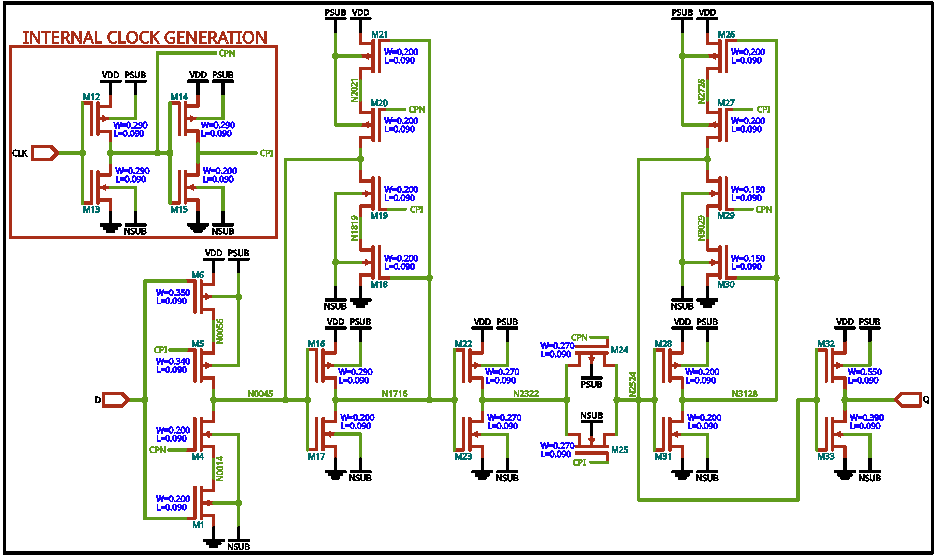
\includegraphics[width=0.5\textwidth]{./figures/CORE65GPSVT_HS65_GS_DFPQX4.pdf}
	\caption{DFF MOS SCH \textcolor{red}{A-T-ON LE DROIT DE METTRE CE SCHÉMA ?}}
\end{figure}

	The complete DFF schematic is shown in Fig. \ref{dffmos}.
	
	The significant extracted signals are the following:
	\begin{itemize}
		\item VDD: the power supply voltage;
		\item VSS: the power supply reference voltage;
		\item PSUB: the bulk voltage of the PMOS transistors;
		\item NSUB: the bulk voltage of the NMOS transistors.
	\end{itemize}
	The voltages PSUB and NSUB depend on the substrate type.
